\documentclass[]{article}
\usepackage{caption,subcaption,graphicx,float,url,amsmath,amssymb,amsthm,tocloft,cancel,thmtools}
\usepackage[toc,nonumberlist]{glossaries}
\usepackage{glossaries-extra}
\newcommand\numberthis{\addtocounter{equation}{1}\tag{\theequation}}
\newtheorem{defn}{Definition}
\newtheorem{thm}{Theorem}
\newtheorem{lemma}[thm]{Lemma}
\graphicspath{{figs/}}
\widowpenalty10000
\clubpenalty10000

\makeglossaries

%opening
\title{
	Theoretical Minimum\\
	Statistical Mechanics
}

\author{Simon Crase}

\begin{document}

\newglossaryentry{gls:adiabatic}{
	name={adiabatic},
	description={
		An adiabatic process is a process in which the entropy doesn’t
		change.}}

\newglossaryentry{gls:exact}{
	name={exact},
	description={
		If $\frac{\partial G}{\partial y} = \frac{\partial H}{\partial x}$, we say that the differential form $dF = G dx + H dy$ is exact.}}
	
\newglossaryentry{gls:heat_capacity}{
	name={heat capacity},
	description={$C_V \triangleq \frac{\partial}{\partial T} \langle E \rangle$},
	symbol=\ensuremath{C_V}}
	
\newglossaryentry{gls:helmholtz}{
	name={Helmholtz Free Energy},
	description={Thermodynamic potential that measures the useful work obtainable from a closed thermodynamic system at a constant temperature and volume $A\triangleq E - TS$ },
	symbol=A}

\newglossaryentry{gls:phase:transition} {
	name={phase transition},
	description={
		The term phase transition (or phase change) is most commonly used to describe transitions between solid, liquid, and gaseous states of matter, as well as plasma in rare cases. A phase of a thermodynamic system and the states of matter have uniform physical properties. During a phase transition of a given medium, certain properties of the medium change, often discontinuously, as a result of the change of external conditions, such as temperature, pressure, or others. For example, a liquid may become gas upon heating to the boiling point, resulting in an abrupt change in volume.}}
	
\maketitle

\begin{abstract}
These are my notes from the Statistical Mechanics lectures from Leonard Susskind's Theoretical Minimum series.
\end{abstract}

\tableofcontents

\listoffigures

\listoftheorems[ignoreall,onlynamed]

\section{Entropy and conservation of information}


This lecture focuses on the law of conservation of energy, the $-1^{th}$ law of physics. 

\begin{thm}[Liouville's theorem]
	The phase-space distribution function is constant along the trajectories of the system—-that is that the density of system points in the vicinity of a given system point travelling through phase-space is constant with time.
\end{thm}

\begin{align*}
S \triangleq \log(M) \numberthis \label{eq:entropy:simple}
\end{align*}

Proper laws of physics are reversible and therefore preserve the distinctions between states - i.e. information.  In this sense, the conservation of information is more fundamental than other physical quantities such as temperature or energy.  
\begin{itemize}
	\item $S$ conserved as long as we can follow in detail, e.g. if we can follow the motion of each molecule that is disturbed by Friction.
	\item $S$ increases as our ignorance goes up;
	\item $S$ depends on the system and our state of knowledge.
\end{itemize}

\begin{align*}
S \triangleq - \sum_{i=1}^{N} p_i \log{p_i} \numberthis \label{eq:entropy}
\end{align*}


In (\ref{eq:entropy:simple}) and (\ref{eq:entropy}) we use the logarithm, so that entropy adds rather than multiplies.

The First law of Thermodynamics is energy conservation. For a closed system:
\begin{align*}
\frac{dE}{dt} =& 0\\
\sum \frac{dE_i}{dt} =& 0
\end{align*}


\section{Temperature}


Temperature is really a measure of Energy. So the energy of one molecule of an Ideal Gas is given by:
\begin{align*}
E =& \frac{3}{2} k_B t\text{, where:}\\
k_B =& \text{ Boltzmann's constant}\\
T =& \text{ temperature in Kelvin}
\end{align*}
 In natural units we define a new unit of temperature, $T=k_Bt$, so $k_B=1$.
 
 We want to redefine temperature in terms of Entropy and Energy, and then show that this new definition agrees with our everyday idea of temperature. Temperature is not a fundamental quantity, but is derived as the amount of energy required to add an incremental amount of entropy to a system.  As the energy of a system increases, the number of possible states of a system increases, which means that the entropy increases.  This is the concept behind the second law of thermodynamics; it implies that temperature is always positive.
 
 Our definition reduces to:
\begin{align*}
\Delta E =& \underbrace{\frac{\partial E}{\partial S}}_\text{1 Degree of T} \Delta S\text{,or }\\
dE =& T dS \numberthis \label{eq:T}
\end{align*}

Consider two systems, $A$ and $B$, joined by a narrow pipe. Theorem \ref{thm:heat:flow} shows that T captures our intuition about temperature: heat flows from a higher temperature to lower.

\begin{thm}[Heat flows from higher temperature to lower]\label{thm:heat:flow}
	Given:
	\begin{align*}
	dE_A + dE_B =& 0 \text{, first law of thermodyamics}\numberthis \label{eq:thm:dE}\\
	dS_A + dS_B>& 0 \text{, second law of thermodynamics}\numberthis \label{eq:thm:eS} \\
	dE_i =& T_i dS_i \text{, from (\ref {eq:T})} \numberthis \label{eq:thm:T} \\
	T_A>&T_B \text{, Assumption.}\numberthis \label{eq:thm:Tgt}
	\end{align*}
	then energy flows from A to B, i.e.
	\begin{align*}
	dE_A<0\numberthis \label{eq:heat:flow:demonstrandum}
	\end{align*}
\end{thm}
\begin{proof}
	\begin{align*}
	T_A dS_A =& dE_A \text{, from (\ref{eq:thm:T})}\\
	=& - dE_B \text{, from (\ref{eq:thm:dE})}\\
	=& - T_B dS_B  \text{, from (\ref{eq:thm:T})}\\
	\implies&\\
	T_A dS_A + T_A dS_B =& T_A dS_B -T_B dS_B\\
	\implies&\\
	T_A (dS_A + dS_B) =& (T_A  -T_B) dS_B\\
	\implies& \text{, using (\ref{eq:thm:eS}) and (\ref{eq:thm:Tgt})}\\
	dS_B >& 0\text{, since temperature positive.}\\
	\implies& \text{using (\ref{eq:thm:T})}\\
	dE_B >& 0\\
	\implies& \text{, using (\ref{eq:thm:dE})}\\
	dE_A<&0\text{, which is (\ref{eq:heat:flow:demonstrandum})}
	\end{align*}
\end{proof}



\section{Maximizing entropy}


As the number of particles in a system grows, the distribution of states clumps more tightly around a mean. This is the Maxwell-Boltzmann distribution. The derivation requires Stirling's approximation and Lagrange multipliers.

Assume that we have N particles, and that there are $n_i$ particles in the $i^{th}$ energy level. Then the number of arrangements is given by
\begin{align*}
C\triangleq\frac{N!}{\prod_{i}n_i!} \numberthis \label{eq:number:combinations}
\end{align*}
 We want to maximize this subject to two constraints:
\begin{align*}
\sum_{i=1}^{N} n_i =& N \text{, total number of particles} \numberthis\label{eq:sum:probilities}\\
\sum_{i=1}^{N} E_i n_i =& E N \text{, average energt.}\numberthis\label{eq:total:energy}
\end{align*}

We will find Lemma \ref{lemma:Stirling} useful.
\begin{lemma}[Stirling's approximation]\label{lemma:Stirling}
	\begin{align*}
	N! \approxeq& N^N e^{-N}\numberthis\label{eq:stirling}
	\end{align*}
\end{lemma}

\begin{proof}
	\begin{align*}
	\log(N!) =& \sum_{i=1}^{N}\log (i)\\
	\approxeq &\int_{1}^{N} \log(x) dx\\
	\approxeq& \big[x \log(x) - x \big]_1^N\\
	\approxeq& N\log(N)-N\text{, whence} \\
	N! \approxeq& N^N e^{-N}
	\end{align*}
\end{proof}	

\begin{thm}[Maximum entropy principle.]
	To maximize the number of arrangements we need to maximize the entropy.
\end{thm}

\begin{proof}
	\begin{align*}
	C=&\frac{N!}{\prod_{i}n_i!} \tag*{from (\ref{eq:number:combinations})}\\
	\approxeq& \frac{N^N e^{-N}}{\prod_{i}n_i^{n_i} e^{-\sum_{i=1}^{N}n_i}}\tag*{from Lemma \ref{lemma:Stirling}}\\
	\approxeq& \frac{N^N \bcancel{e^{-N}}}{\prod_{i}n_i^{n_i} \bcancel{e^{-N}}}\tag*{using (\ref{eq:sum:probilities})}\\
	\log(C) \approxeq & N \log(N) - \sum_{i=1}^{N} n_i \log(n_i)\\
	\approxeq& N \log(N) - \sum_{i=1}^{N} N p_i \log(N p_i)\\
	\approxeq& N \log(N) - \sum_{i=1}^{N} N p_i \big(\log(N) + \log(p_i))\big)\\
	\approxeq& N \log(N) -  N \log(N) \bcancel{\sum_{i=1}^{N} p_i}  - N \sum_{i=1}^{N}p_i \log(p_i)\tag*{using (\ref{eq:sum:probilities})}\\
	\approxeq& \bcancel{N \log(N)} - \bcancel{N \log(N)}  - N \sum_{i=1}^{N}p_i \log(p_i)\\
	\approxeq& NS \text{, using (\ref{eq:entropy})} \numberthis \label{eq:entropy:logC}
	\end{align*}
\end{proof}

\section{The Boltzmann distribution}

\subsection{The Boltzmann distribution}

To maximize S subject to constraints (\ref{eq:sum:probilities}) and (\ref{eq:total:energy}), we minimize -S, using Lagrange Multipliers, i.e., minimize
\begin{align*}
\sum_{i=1}^{N}p_i \log(p_i) + \alpha(\sum_{i=1}^{N} p_i-1) + \beta(\sum_{i=1}^{N} E_i p_i-E)\text{, where $\alpha$ and $\beta$ are parameters to be determined.}
\end{align*}

Differentiating with respect to $p_i$:
\begin{align*}
\log(p_i)+1 + \alpha +\beta E_i=&0\text{, whence}\\
p_i =& e^{-(1+\alpha)} e^{-\beta E_i}\\
=& \frac{1}{Z} e^{-\beta E_i}\text{, where $Z\triangleq e^{(1+\alpha)}$} \numberthis\label{eq:maximize:entropy}
\end{align*}

From (\ref{eq:sum:probilities}) and (\ref{eq:maximize:entropy})
\begin{align*}
1 =& \frac{1}{Z}  \sum_{i=1}^{N} e^-{\beta E_i}\\
Z(\beta) =& \sum_{i=1}^{N} e^-{\beta E_i} \text{. $Z$ is known as the Partition Function.} \numberthis \label{eq:partition:function}
\end{align*}

\begin{thm}[$\beta$ is the inverse temperature]\label{thm:inverseT}
	\begin{align*}
		T =& \frac{1}{\beta}\numberthis\label{eq:inverseT}
	\end{align*}
\end{thm}

\begin{proof}
	From (\ref{eq:total:energy}) and (\ref{eq:maximize:entropy})
	\begin{align*}
	E =& \frac{1}{Z}  \sum_{i=1}^{N} e^{-\beta E_i} E_i \text{\, and}\numberthis \label{eq:E}\\
	\frac{\partial Z}{\partial \beta} =& - \sum_{i=1}^{N} e^{-\beta E_i} E_i \text{, from (\ref{eq:partition:function}), whence} \numberthis \label{eq:dZ}\\
	E(\beta) =& - \frac{1}{Z} \frac{\partial Z}{\partial \beta} = - \frac{\partial \log(Z)}{\partial \beta} \numberthis \label{eq:E:beta}
	\end{align*}
	
	\begin{align*}
	S =& -\sum_{i=1}^{N} p_i \log(p_i) \text{, from (\ref{eq:entropy})}\\
	=& - \sum_{i=1}^{N} \frac{1}{Z} e^{- \beta E_i}\big[- \beta E_i -\log(Z)\big]\text{, from (\ref{eq:maximize:entropy})}\\
	=& \beta E +  \bcancel{\frac{1}{Z}} \log(Z)  \bcancel{\sum_{i=1}^{N} e^{-\beta E_i}}\\
	=& \beta E +   \log(Z)  \numberthis \label{eq:S_Z}
	\end{align*}
	
	\begin{align*}
	dS =& \beta dE + E d\beta + \frac{\partial \log(Z)}{\partial \beta} d\beta \text{, from (\ref{eq:S_Z})}\\
	=& \beta dE \text{, using (\ref{eq:E:beta})}\\
	=& \frac{1}{T} dE \text{, using (\ref{eq:T})}\text{, whence}\\
	T =& \frac{1}{\beta}
	\end{align*}
\end{proof}

\subsection{Ideal Gas}.

We will find the following theorem useful.

\begin{thm}[Gaussian Integral]\label{thm:gaussian_integral}
	\begin{align*}
		\int_{-\infty}^{\infty} e^{-a^2 x^2} dx = \frac{\sqrt{\pi}}{a}
	\end{align*}
\end{thm}

\begin{proof}
	\begin{align*}
		\int_{-\infty}^{\infty} e^{-a^2 x^2} dx =& \frac{1}{a} \int_{-\infty}^{\infty} e^{-(ax)^2} d(ax) \\
		=& \frac{1}{a} \int_{-\infty}^{\infty} e^{-z^2} dz \numberthis \label{eq:gauss_a}\\
		\int_{-\infty}^{\infty} e^{-x^2} dx \int_{-\infty}^{\infty} e^{-y^2} dy =& \int_{-\infty}^{\infty} \int_{-\infty}^{\infty} e^{-(x^2+y^2)}  dx dy\\
		=& \int_0^{2\pi} \int_{0}^{\infty}e^{-r^2} r dr d\theta\\
		=& \int_0^{2\pi}  d\theta  r dr\\
		=& 2\pi \int_{0}^{\infty}e^{-(r^2)} \frac{1}{2} d(r^2)\\
		=& \pi \int_{0}^{\infty} e^{-z} dz\\
		=& - \pi  e^{-z}\bigg\vert_{z=0}^{\infty}\\
		=& \pi\text{, whence}\\
		\int_{-\infty}^{\infty} e^{-x^2} dx =& \sqrt{\pi}\text{. Using \ref{eq:gauss_a}}\\
		\int_{-\infty}^{\infty} e^{-a^2 x^2} dx =& \frac{\sqrt{\pi}}{a}
	\end{align*}
\end{proof}

Assume molecules don't interact. State consists of 6N coordinates,  $\{X_1,...X_{3N}\}$ and momenta $\{P_1,...P_{3N}\}$. From (\ref{eq:partition:function})
\begin{align*}
Z =& \int d^{3N}x d^{3N}p . e^{- \frac{\beta}{2m} \sum_{n=1}^{3N} p_n^2}\\
=& \frac{V^N}{N!} \int d^{3N}p . e^{- \frac{\beta}{2m} \sum_{n=1}^{3N} p_n^2}\textit{--Factorial is controversial}\\
=& \frac{V^N}{N!} \big[\int dp. e^{-\frac{\beta}{2m}p^2}\big]^{3N}\\
=& \frac{V^N}{N!} \big[\frac{2 m \pi}{\beta}\big]^{\frac{3N}{2}}\numberthis\label{eq:Z_beta}\text{, from Theorem \ref{thm:gaussian_integral}}
\end{align*}
We now use Stirling's formula (\ref{eq:stirling}).
\begin{align*}
\frac{V^N}{N!} \approxeq& \big(\frac{eN}{N}\big)^N \\
=& \big(\frac{e}{\rho}\big)^N,\text{, and (\ref{eq:E:beta}) becomes}\\
Z \approxeq& \big(\frac{e}{\rho}\big)^N .  \big[\frac{2 m \pi}{\beta}\big]^{\frac{3N}{2}}
\end{align*}

\begin{align*}
\log(Z) =& - \frac{3N}{2} \log(\beta) + const\\
E =& - \frac{\partial \log(Z)}{\partial \beta}\numberthis \label{eq:E:Z}\\
=& \frac{3N}{2} T
\end{align*}


\section{Pressure of an ideal gas and fluctuations}

\subsection{Pressure of an ideal gas}

\begin{itemize}
	\item Motion is isotropic, even near wall. We know this from an honest use of statistical mechanics.
	\item Give up intuition because it might not be correct ''ride the mathematics''.
	\item Question : Once we have done the mathematics of a pro-
	blem, can’t we check them with our intuition?
	\item Answer : Yes we can, but what we are really doing is che-
	cking our intuition not the mathematics.
	\item All very great physicists are master of thermodynamics.''
\end{itemize}

We want to determine the Equation of State.

From (\ref{eq:S_Z}) and Theorem \ref{thm:inverseT}.
\begin{align*}
S =& \frac{E}{T} + \log(Z)\\
A\triangleq &E - TS\tag*{Helmholtz Free Energy} \\
=& -T \log(Z) \numberthis \label{eq:helmholtz}
\end{align*}



Variables come in pairs, e.g. (V,P):
\begin{itemize}
	\item Control Parameter--a parameters that w, as experimenters, can easily change. They are macroscopic parameters: we are not trying to change details of one molecule at a time. V is a control parameter;
	\item Conjugate Thermodynamic Variable (P).
\end{itemize}

\begin{lemma}[Derivatives along contour]\label{thm:derivative:contour}
	Given two dependent variables, S and E, say, and two independent variables, T and V, say:
	\begin{align*}
		\frac{\partial E}{\partial V}\bigg|_S = \frac{\partial E}{\partial V}\bigg|_T - 	\frac{\partial E}{\partial S}\bigg|_V \frac{\partial S}{\partial V}\bigg|_T
	\end{align*}
\end{lemma}
\begin{proof}
	Along a contour of fixed S:
	\begin{figure}[H]
		\caption{$E(B)-E(A) = \big[E(C)-E(A)\big]+\big[E(B)-E(C)\big]$}\label{fig:contour:of:fixed:S}
		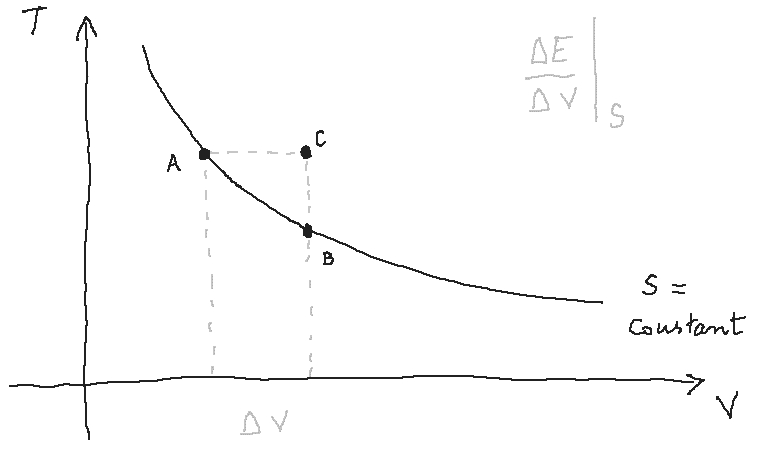
\includegraphics[width=0.9\textwidth]{partial-derivatives}
	\end{figure}
	\begin{align*}
		\Delta E =& \frac{\partial E}{\partial V} \bigg|_T \Delta V + \frac{\partial E}{\partial T} \bigg|_V \Delta T \text{, by inspecting Figure \ref{fig:contour:of:fixed:S}. The $2^{nd}$ term gives:}\\
		\frac{\partial E}{\partial T} \bigg|_V \Delta T=& \frac{\partial S}{\partial T} \bigg|_V \frac{\partial E}{\partial S} \bigg|_V \Delta T\text{, whence:}\\
		\frac{\partial E}{\partial V} \bigg|_S=& \frac{\partial E}{\partial V} \bigg|_T  + \frac{\partial S}{\partial T} \bigg|_V \frac{\partial E}{\partial S} \bigg|_V \frac{\Delta T}{\Delta V} \numberthis\label{eq:dEdV}\\
		\text{Now }\Delta S =& \frac{\partial S}{\partial V} \bigg|_T \Delta V + \frac{\partial S}{\partial T} \bigg|_V \Delta T\\
		=& 0\text{, along a contour of constant S, whence}\\
		\frac{\Delta T}{\Delta V} =& - \Bigg[\frac{\frac{\partial S}{\partial V}\big|_T}{\frac{\partial S}{\partial T}\big|_V}\Bigg]\text{, along a contour of constant S, so (\ref{eq:dEdV}) becomes:}\\
		\frac{\partial E}{\partial V} \bigg|_S=& \frac{\partial E}{\partial V} \bigg|_T  - \cancel{\frac{\partial S}{\partial T} \bigg|_V} \frac{\partial E}{\partial S} \bigg|_V \frac{\frac{\partial S}{\partial V}\big|_T}{\cancel{\frac{\partial S}{\partial T}\big|_V}}\\
		=& \frac{\partial E}{\partial V} \bigg|_T  -  \frac{\partial E}{\partial S} \bigg|_V \frac{\partial S}{\partial V}\bigg|_T
	\end{align*}
\end{proof}

NB. For most situations, S is a monotonic increasing function of E. As E increases, distribution gets broader, and S increases. 

\begin{figure}[H]
	\caption{Imagine piston is vertical}\label{fig:vertical:piston}
	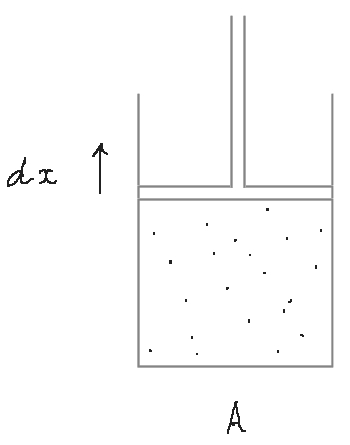
\includegraphics[width=0.9\textwidth]{vertical-piston}
\end{figure}

Imagine piston is vertical.

\begin{itemize}
	\item Move piston out, gas does work, which is paid for from energy.
	\item Move piston in, we do work, which adds to energy.
\end{itemize}

Move piston slowly, and don't let energy in. Adiabatic: slowly, and no heat in or out. $dE = - P \mathcal{A}dx$, where $\mathcal{A}$ is the area of the piston in Figure \ref{fig:vertical:piston}. Since $\mathcal{A}dx = dV$, $dE = -P dV$. 

\begin{align*}
\frac{\partial E}{\partial V}\bigg|_S =& - P\numberthis \label{eq:defP}
\end{align*}

\begin{figure}[H]
	\caption{Energy Levels as a function of volume}
	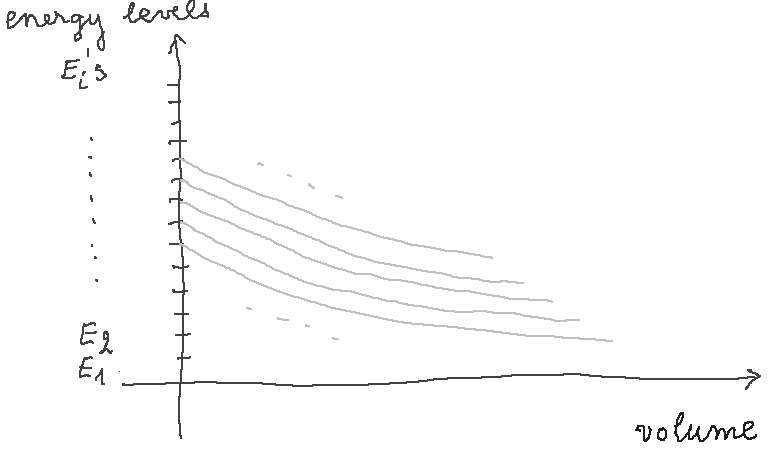
\includegraphics[width=0.9\textwidth]{energy-levels-volume}
\end{figure}




\begin{thm}[Adiabatic Theorem]\label{thm:adiabatic}
	Change volume \gls{gls:adiabatic}ally, the system will ride along the energy level: it will change, but not jump.
\end{thm}

\begin{itemize}
	\item One consequence of Theorem \ref{thm:adiabatic} is that the $p_i$ are fixed.
	
	\item Isentropic is also adiabatic.
	
	\item Easier to use T as it appears in Bolzmann.
\end{itemize}

\begin{align*}
P =& - \frac{\partial E}{\partial V}\bigg|_S \\
=& - \frac{\partial E}{\partial V}\bigg|_T + \frac{\partial S}{\partial V}\bigg|_T \frac{\partial E}{\partial S}\bigg|_V\text{, from Lemma \ref{thm:derivative:contour}}\\
=& - \frac{\partial E}{\partial V}\bigg|_T + \frac{\partial S}{\partial V}\bigg|_T T\text{, from (\ref{eq:T})}\\
=& - \frac{\partial(E-TS)}{\partial V}\bigg|_T \text{, from (\ref{eq:helmholtz})--\gls{gls:helmholtz}} \glssymbol{gls:helmholtz}\\
=& T \frac{\partial \log(Z)}{\partial V}\bigg|_T \numberthis \label{eq:P_Z_V}
\end{align*}

\begin{itemize}
	\item We haven't used assumption that we are dealing with a gas, so this is completely general.
	\item could have used different conjugate pair.
\end{itemize}

The partition function is given by:
\begin{align*}
Z(\beta) =& \int dx dp e^{- \beta \frac{p^2}{2m}}\\
=& \frac{V^N}{N!} f(\beta)\\
\log(Z) =& N \log(V) + \log(f(\beta))\text{, so (\ref{eq:P_Z_V})  becomes:}\\
P =& \frac{NT}{V}\text{, or}\\
P =& \rho T
\end{align*}

\subsection{Fluctuations}

\begin{align*}
	\langle E -  \langle E \rangle \rangle^2 =& \langle E^2 \rangle - \langle E \rangle^2\text{. Now, from (\ref{eq:E:beta})}\\
	\langle E \rangle=& - \frac{\partial \log(Z)}{\partial \beta}\text{, and from (\ref{eq:dZ})}\\
	 \langle E^2 \rangle =& \frac{1}{Z} \frac{\partial^2 Z}{\partial \beta^2} \text{, whence}\\
	 \langle E^2 \rangle =& \frac{1}{Z} \frac{\partial^2 Z}{\partial \beta^2} - \frac{1}{Z^2} \bigg(\frac{\partial Z}{\partial \beta}\bigg)^2 \numberthis \label{E2Z}
\end{align*}
All of statistical mechanics is about the power of the partition function.



\begin{align*}
	\frac{\partial^2 \log(Z)}{\partial \beta^2} =& \frac{\partial}{\partial \beta} \frac{1}{Z} \frac{\partial Z}{\partial \beta}\\
	=& \frac{1}{Z} \frac{\partial^2 Z}{\partial \beta^2} - \frac{1}{Z^2} \bigg(\frac{\partial Z}{\partial \beta}\bigg)^2\\
	(\Delta E)^2 =& \frac{\partial}{\partial \beta} \frac{1}{Z} \frac{\partial Z}{\partial \beta}\text{, from (\ref{E2Z})}\\
	=& - \frac{\partial}{\partial \beta} \langle E \rangle\\
	=&  \frac{\partial}{\partial T} \langle E \rangle T^2 \tag*{from (\ref{eq:inverseT})}\\
	=& C_V T^2\text{, where} \numberthis \label{eq:einstein:gibbs}\\
	C_V \triangleq& \frac{\partial}{\partial T} \langle E \rangle \text{, \Gls{gls:heat_capacity}}
\end{align*}



\begin{itemize}
	\item (\ref{eq:einstein:gibbs}) is due to Einstein and Gibbs.
	\item True for any system: we haven't assumed ideal gas.
\end{itemize}


\section{Weakly interacting gases, heat, and work}


\subsection{Weakly interacting gases}

We will assume:
\begin{itemize}
	\item dilute;
	\item molecules on average far from each other;
	\item range of forces small compared to distance between particles;
	\item potential energy or forces small.
\end{itemize}

Then we will ask where this breaks down; where does correction becomes as large as uncorrected. 

We calculate partition function for a system where total energy not equal to sum of kinetic energies.

Assume energy has the following form:
\begin{align*}
E =& \sum_{n} \frac{p^2}{2M} + \underbrace{\sum_{n>m}u(\vert(x_m-x_n)\vert)}_{U(x)\text{, say}}
\end{align*}
, where $u$ is small compared to kinetic energy, and define:
\begin{align*}
U_0 \triangleq& \int d^3x x.u(\vert x \vert)\text{, then}\\
\int d^3x_1 d^3s_2 u(\vert x_1 - x_2\vert) = & V U_0\text{, ignoring surface expects!}
\end{align*}
NB: $U$ factors in collisions!

\begin{align*}
Z =& \int \frac{dp dx}{N!} e^{- \beta \frac{p^2}{2M}} e^{-\beta U(x)}\\
=&\underbrace{ \int \frac{dp}{N!} e^{- \beta \frac{p^2}{2M}}}_{\Big(\sqrt{\frac{2\pi m}{\beta}}\Big)^3} \int dx.e^{-\beta U(x)}\\
=&\underbrace{ \int \frac{dp.V^N}{N!} e^{- \beta \frac{p^2}{2M}}}_{\text{Partition function for Ideal Gas}} \int dx.\frac{e^{-\beta U(x)}}{V^N}\\
=&Z_0(\beta) \int dx.\frac{e^{-\beta U(x)}}{V^N}\text{ say.}\numberthis \label{eq:introducingZ0}\\
\int dx.\frac{e^{-\beta U(x)}}{V^N}\approxeq& \int \frac{dx}{V^N} \Big(1 - \beta U(x)\Big)\text{, assuming U small}\\
\approxeq & 1 - \beta \int \frac{dx}{V^N} U(x)\\
\approxeq & 1 - \beta \int \frac{dx}{V^N} \sum_{n>m} u(\vert x_n - x_m\vert)\\
\approxeq & 1 - \frac{N(N-1)\beta}{2} \int \frac{dx_1.dx_2}{V^N}  u(\vert x_1 - x_2\vert) V^{N-2}\\
\approxeq& 1 - \frac{N^2}{2}\beta \frac{U_0}{V}\\
Z \approxeq& Z_0(\beta) \Big[1 - \frac{\beta N^2}{2V} U_0\Big]
\end{align*}

\begin{align*}
\log(Z) =& \log(Z_0) + \log\Big[1 - \frac{\beta N^2}{2V} U_0\Big] \\
\approxeq & \log(Z_0) - \frac{\beta N^2}{2V} U_0\\
E =& - \frac{\partial \log Z}{\partial \beta}\\
=& \frac{3}{2}NT + \frac{N^2}{2V}U_0\\
=& \Big[\frac{3}{2}T + \frac{ \rho}{2}U_0\Big] N
\end{align*}

Since E is difficult to measure, we'll also calculate P. From (\ref{eq:P_Z_V}).

\begin{align*}
P =& T \frac{\partial \log(Z)}{\partial V}\bigg|_T\\
=& \rho T + \frac{\rho^2}{2} U_0\text{, provided $\rho U_0 \ll T$, i.e. potential energy much less than kinetic energy.}
\end{align*}

\subsection{Heat \& Work}

We shall find the following theorem useful.

\begin{thm}[Clairaut-Schwarz]\label{thm:2partial}
	If $\frac{\partial^2 F}{\partial x \partial y}$ and $\frac{\partial^2 F}{\partial y \partial x}$ both exist and are continuous at some point $(x_0,y_0)$, then there exists a neighbourhood of $(x_0,y_0)$ where:
	\begin{align*}
	\frac{\partial^2 F}{\partial x \partial y} = \frac{\partial^2 F}{\partial y \partial x}
	\end{align*}
\end{thm}


Given $F(x,y)$
\begin{align*}
dF =& \frac{\partial F}{\partial x}dx + \frac{\partial F}{\partial y}dy\\
=& G dx + H dy\text{, say}\numberthis \label{eq:dF}\\
\frac{\partial G}{\partial y} =& \frac{\partial H}{\partial x}\text{, using Theorem \ref{thm:2partial}}\numberthis \label{eq:exact}
\end{align*}

\glsdesc{gls:exact}

 
Consider an adiabatic change to system of cylinder and piston.

\begin{align*}
dE =& -P dV \text{, change V only}\\
=& T dS \text{, hold V, add heat}\\
=& \underbrace{-P dV}_{dW} + \underbrace{T dS}_{dQ}\text {, change both. First Law of Thermodynamics}
\end{align*}

Is $dQ$ an exact differential?

\begin{align*}
dQ =& dE + P.dV\text{. If exact}\\
\frac{\partial Q}{\partial E}=&1, \frac{\partial Q}{\partial V} = P\\
\frac{\partial^2 Q}{\partial V \partial E} \ne& \frac{\partial^2 Q}{\partial E \partial V}\text{, so $dQ$ is not exact.}
\end{align*}

\section{Entropy vs. reversibility}

\subsection{The speed of sound in an ideal gas}

Create a small overdense region. How fast does it move out? With the average velocity of molecules.

In thermal equilibrium in a dilute gas, every molecule has velocity $v$
\begin{align*}
\frac{3}{2} k_B T =& \frac{m}{2} v^2\text{ We'll use laboratory units, so $k_B$}\\
v^2 =& \frac{3 k_B T}{m}\text{. A more detailed analysis gives:} \numberthis \label{eq:c:rough}\\
c^2 =& \frac{1}{m}\frac{\partial P}{\partial \rho} \text{, where $c$ represents speed of sound (not light)}\\
P =& \rho k_B T\text{ Ideal gas law}\\
\implies&\\
c^2 =& \frac{k_B T}{m}\text{. (\ref{eq:c:rough}) is within order of magnitude!}
\end{align*}


\subsection{A single harmonic oscillator in a heat bath}

\begin{align*}
Energy =& \frac{m}{2} \dot{x}^ 2 + \frac{k}{2} x^2\tag{ $k$ is not Boltzmann!}\\
=& \frac{1}{2m} p^ 2 + \frac{k}{2} x^2\\
Z(\beta) =& \int e^{-\beta \frac{1}{2m} p^ 2 } e^{-\beta \frac{k}{2} x^2} dp dx\\
=& \int e^{-\beta \frac{1}{2m} p^ 2 } dp \int e^{-\beta \frac{k}{2} x^2} dx\\
=& \sqrt{\frac{2m\pi}{\beta}}\sqrt{\frac{2 \pi}{\beta k}} \text{, using Theorem \ref{thm:gaussian_integral}}\\
=& \frac{2 \pi}{\omega}\frac{1}{\beta}\text{, where} \numberthis\label{eq:Z:classical:q}\\
\omega =& \sqrt{\frac{k}{m}} \text{ represents the frequency. Now}\\
\log(Z) =& \log(2\pi) -\log(\omega) - \log(\beta)\text{, whence }\\
E =& - \frac{\partial \log(Z)}{\partial \beta}\text{, from (\ref{eq:E:Z})}\\
=& \frac{1}{\beta}\\
=& T \text{, from Theorem \ref{thm:inverseT}}
\end{align*}

\begin{itemize}
	\item Why no 3? Because 1 dimensional.
	\item Why not 2? Because 2 integrals.
\end{itemize}

Note:
\begin{itemize}
	\item Energy doesn't depend on $m$;
	\item Energy doesn't depend on $k$. This seems wrong (make $k$ very large). This was a big problem around the end of 19th century (what about diatomic molecules 3 becomes 5?) We have ignored quantum mechanics!
\end{itemize}



\begin{align*}
	Z(\beta) =& \sum_{n} e^{- \beta n \hbar \omega}\\
	 =& \sum_{n} \Big(e^{- \beta\hbar \omega}\Big)^n\\
	 =& \frac{1}{1 - e^{- \beta\hbar \omega}}\numberthis\label{Z_quantum_shm}\\
	 E =& - \frac{1}{Z} \frac{\partial Z}{\partial \beta}\\
	 \frac{\partial Z}{\partial \beta}=& \frac{- \hbar \omega e^{- \beta\hbar \omega}}{(1 - e^{- \beta\hbar \omega})^2}\\
	 E =& \frac{ \hbar \omega e^{- \beta\hbar \omega}}{(1 - e^{- \beta\hbar \omega})}
\end{align*}

High temperature: $T\rightarrow\infty \implies \beta \rightarrow 0$
\begin{align*}
	\frac{ \hbar \omega e^{- \beta\hbar \omega}}{(1 - e^{- \beta\hbar \omega})}\rightarrow& \frac{\hbar \omega}{1 -(1 - \beta \hbar \omega...)}\\
	\rightarrow& \frac{\hbar \omega}{\beta \hbar \omega}\\
	\rightarrow& \frac{1}{\beta}\\
	\rightarrow& T\text{, which agrees with classical physics.}
\end{align*}

Low temperature: $T\rightarrow 0 \implies \beta \rightarrow \infty$

\begin{align*}
\frac{ \hbar \omega e^{- \beta\hbar \omega}}{(1 - e^{- \beta\hbar \omega})}\rightarrow&\hbar \omega e^{- \beta\hbar \omega}\\
\rightarrow&0
\end{align*}

So for low temperature, oscillation is suppressed.	Where is the crossover between classical and quantum behaviour? This occurs when exponential goes from large to small (and vice versa), i.e. when $\beta\hbar \omega \approx 1$.

\begin{itemize}
	\item $\beta\hbar \omega < 1$ Classical.
	\item $\beta\hbar \omega > 1$ Quantum.
	\item $\beta\hbar \omega = 1\equiv\hbar \omega=T$ Crossover. At this temperature, system has one quantum of energy; it doesn't want to have less!
	\item For very low temperature, diatomic molecule behaves like monoatomic.
	\item For a stiff molecule, $\omega$ is high, so crossover temperature is high.
\end{itemize}

c.f. Einstein specific heat.

Can we derive classical partition function from quantum?

\begin{align*}
Z(\beta) =&  \frac{1}{1 - e^{- \beta\hbar \omega}} \text{, from (\ref {Z_quantum_shm})}\\
\approxeq & \frac{1}{1 - 1 + \beta\hbar \omega}\text{, for high T}\\
\approxeq & \frac{1}{\beta\hbar \omega}\text{, c.f. (\ref{eq:Z:classical:q})}
\end{align*}

\begin{itemize}
	\item So the classical and quantum partition functions agree within a multiplicative constant, which disappears when we differentiate $\log(Z)$ to do anything useful.
	\item Heat system: it unfreezes degrees of freedom and we discover complexity. Cool system: discover quantum behaviour.
	\item Violin string: freeze out higher frequency states, so energy finite.
\end{itemize}

\subsection{Contradiction between the 2nd and reversibility}
\begin{itemize}
	\item Newton's laws reversible
	\item 2nd law of thermodynamics is not reversible!
	\item Consider a small blob in phase space: according to Liouville's theorem, volume, and hence entropy, does not change! Correct view of microscopic system.
	\item We need to coarse grain. Resolution is limited, both by QM, and by our instruments.
	\item Imagine that blob turns into long thing snake (same volume), but we can't resolve, so we cover with blobs. We are now losing information. 
	\item Chaos! Sensitive dependence on initial conditions. Imagine phase space filled with cotton!
	
	\item Phase space trajectory will eventually come back to starting point within specified tolerance: time depends on tolerance.
	
	\item Entropy probably increases -- Boltzmann. 
\end{itemize}


\section{Entropy, reversibility, and magnetism}

\subsection{2nd Law and Poincar\'e Recurrences}

Imagine room with all particles of air in one half. In 6N dimensional phase space, momentum is bounded because we have finite energy. Phase point moves chaotically. Phase point $\frac{1}{2^N}$. Or, imagine configuration space has N dimensions, and is of volume $V^N$; what is probability of finding system in smaller volume $v^N$? $\frac{v^N}{V^N}$. 

\begin{thm}[Poincar\'e Recurrences]
	Any dynamical system defined by an ordinary differential equation determines a flow map $f^t$ mapping phase space on itself. The system is said to be volume-preserving if the volume of a set in phase space is invariant under the flow. For instance, all Hamiltonian systems are volume-preserving because of Liouville's theorem. The theorem is then: If a flow preserves volume and has only bounded orbits, then for each open set there exist orbits that intersect the set infinitely often.
\end{thm}

\begin{proof}
	The proof, speaking qualitatively, hinges on two premises:
	
	\begin{itemize}
		\item 	A finite upper bound can be set on the total potentially accessible phase space volume. For a mechanical system, this bound can be provided by requiring that the system is contained in a bounded physical region of space (so that it cannot, for example, eject particles that never return) – combined with the conservation of energy, this locks the system into a finite region in phase space.
		\item The phase volume of a finite element under dynamics is conserved. (for a mechanical system, this is ensured by Liouville's theorem)
	\end{itemize}
	
	Imagine any finite starting volume of phase space and follow its path under dynamics of the system. The volume "sweeps" points of phase space as it evolves, and the "front" of this sweeping has a constant size. Over time the explored phase volume (known as a "phase tube") grows linearly, at least at first. But, because the accessible phase volume is finite, the phase tube volume must eventually saturate because it cannot grow larger than the accessible volume. This means that the phase tube must intersect itself. In order to intersect itself, however, it must do so by first passing through the starting volume. Therefore, at least a finite fraction of the starting volume is recurring.
	
	Now, consider the size of the non-returning portion of the starting phase volume – that portion that never returns to the starting volume. Using the principle just discussed in the last paragraph, we know that if the non-returning portion is finite, then a finite part of the non-returning portion must return. But that would be a contradiction, since any part of the non-returning portion that returns, also returns to the original starting volume. Thus, the non-returning portion of the starting volume cannot be finite and must be infinitely smaller than the starting volume itself.
\end{proof}
Boltzmann's Brain: most of the ways we could have gotten here are by random fluctuation, and they don't have coherent histories.


\subsection{Magnetism}

A normal magnet is made up of lots of little magnets (atoms). At a high enough temperature, orientation is random. If we cool it down, we get small domains: same direction within domain. Domains start to grow, may have ferromagnetic transition.

$N$ simple magnets, either up or down. Assume magnetic field, no interaction. Spin up, $\sigma(1).$

\begin{align*}
E=&(n-m)\mu H\text{, where n are up, m down, $m+n=N$}\\
\text{number of states} =&\frac{N!}{n!m!}\\
Z =&\sum_{mn\mid m+n=N} e^{- \beta \mu H(n-m)}\\
=&\sum_{n}\frac{N!}{n!(N-n)}X^nY^{N-n}\text{, where $X=e^{-\beta\mu H},Y=e^{\beta\mu H}$}\\
=&\big(X+Y\big)^N\tag*{from the Binomial Theorem}\\
=&\big(e^{-\beta\mu H}+e^{\beta\mu H}\big)^N\\
=&2^N \big(\cosh(\beta\mu H)\big)^N\tag*{Definition of cosh}
\end{align*}

NB: biased by magnetic field!

\begin{align*}
	M \triangleq& \big< \frac{n-m}{N}\big>\text{, Magnetization} \\
	E =& M N \mu H\\
	=& \frac{\partial \log(Z)}{\partial \beta} \text{, from (\ref{eq:E:beta})}\\
	=& - N \frac{\sinh(\beta\mu H)}{\cosh(\beta\mu H)} \mu H\\
	M=& \tanh(\beta\mu H)
\end{align*}

Figure \ref{fig:tanh} show that $M$ is zero for $\beta=0$ (high temperature) and one for large $\beta$ (small temperature).

\begin{figure}[H]
	\caption{Graph of $\tanh$}\label{fig:tanh}
	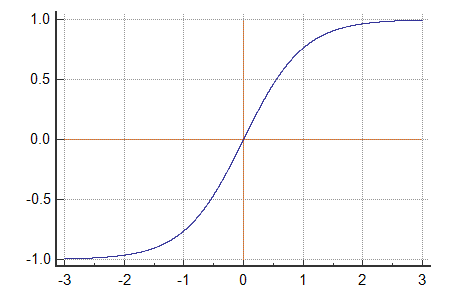
\includegraphics[width=0.8\textwidth]{tanh}
\end{figure}

The Ising model
\begin{align*}
E =& - j \sum_{n} \sigma(n) \sigma(n+1)
\end{align*}

\begin{itemize}
	\item Two ground states
	\item tiniest external magnetic field will bias
	\item spontaneous symmetry breaking
\end{itemize}


\section{The Ising model}

\subsection{One-dimensional Ising model}

Consider one spin in a heat bath, so we can focus on one at a time

\begin{align*}
E =& -j \sigma \text{, where $j=\mu B$}\\
Z =& \sum_{\sigma=\pm 1} e^{-\beta j \sigma}\\
=& e^{\beta j}+ e^{- \beta j}\\
=& 2 \cosh(\beta j) \numberthis \label{eq:E:cosh:beta:j}\\
\big<E\big> =& - \frac{\partial \log(Z)}{\partial \beta}\text{, from (\ref{eq:E:beta})}\\
=& - j \tanh{\beta j}\\
\big<\sigma\big> =& - \tanh{\beta j}
\end{align*}

Figure \ref{fig:tanh} shows that spin points up for $\beta\rightarrow\infty$, so spin parallel to j for low temperature; spin all over the place at high temperature.

Now consider a line of spins. We will assume a specific spin is up, and ask about correlation with some other spin $\big<\sigma(i) \sigma(i+n)\big>$. Assume first spin is up, and focus on relationships, $\mu_i\triangleq\sigma_i\sigma_{i+1}$ (state of link).\footnote{NB: if we reverse the sign of $j$ and reverse the sign of every $2_{nd} \sigma_i$, we get the same problem. }

\begin{align*}
E =& -j \sum_i \sigma_i \sigma_{i+1}\\
=& -j \sum_{b} \mu_b\\
Z =& \sum_{\sigma} e^{- j \beta\sum_i  \sigma_i \sigma_{i+1}} \text{, Partition function}\\
=& 2 \sum_{\mu} e^{- j \beta  \sum_b \mu_b} \text{, allowing for $\sigma_1$}\\
=& \big(2 \cosh(\beta j)\big)^{N-1}\text{, by the same argument as (\ref{eq:E:cosh:beta:j})--}\numberthis \label{eq:Z:cosh} 
\end{align*}

\begin{align*}
\big< \mu \big> =& \big< \sigma_i \sigma_{i+1} \big>\\
=& \tanh(\beta j) \textit{, prove this!}\text{ Correlation between neighbours}\numberthis \label{eg:Z_cosh}
\end{align*}

\begin{align*}
\big < \sigma_i \sigma_{i+n} \big> =&  \big < \sigma_i \sigma_{i+1} \sigma_{i+1}... \sigma_{i+n} \big>\text{, since $\sigma_i^2 = 1$}\\
=& \mu_1 \mu_2 ... \mu_{n-1}\\
=& \big( \tanh(\beta j)\big)^{n-1}\text{, from (\ref{eg:Z_cosh}), since $\mu_i$ independent}
\end{align*}

If $T=0(\beta=\inf)$, $\tanh(..)=\pm1$, otherwise $\lvert \tanh(..) \rvert<1$ and $\tanh(..)^n$ becomes arbitrarily small as $n$ increases.

\begin{itemize}
	\item Note the duality. We have found an equivalence between system of links and system of spins. 
	\item We also see that there can be no magnetization in 1 dimensional system, except for $T=0$. C.f. "Chinese whispers". Likely to be long chains of agreement, then switch.
\end{itemize}
 

\subsection{Phase transitions in the Ising model}

There is no \gls{gls:phase:transition} in the 1D Ising model. For two or more dimensions, there are several paths along which information about one site can propagate, so "Chinese whispers" might not apply.

We will use a "mean field" approximation. In $d$ dimensions, where $d$ is very large, each site has $2d$ neighbours. We expect fluctuations to be much smaller than actual value. Let us assume bias; average spin is $\bar{\sigma}$.

\begin{align*}
E =& -j \sigma \sum_{neighbours} \sigma_{neighbour} \text{, for one spin.}\\
=& -j \sigma \sum_{neighbours} \bar{\sigma}\text{, where $\bar{\sigma}$ is average: mean field approximation.}\\
\approxeq &-2 d j \sigma \bar{\sigma}\text{. This gets more accurate as $d$ increases.} \numberthis \label{eq:E:sigma}\\
Z =& 2 \cosh(\beta 2 d j \bar{\sigma}) \text{--compare (\ref{eq:Z:cosh})}\\
\bar{\bar{\sigma}} =& \tanh\big(\underbrace{2 \beta d j  \bar{\sigma}}_\text{$=y$, say}\big) \text{, where $\bar{\bar{\sigma}}$ is expected $\sigma$} \\
\bar{\bar{\sigma}} =& \bar{\sigma} \text{, ''self-consistent'' approximation. We now solve:}\\
\frac{T y}{2 d j} =& \tanh(y)\numberthis \label{eq:tanh_mean_field}
\end{align*}  

Figure \ref{fig:tanh_mean_field} exhibits a phase-transition at $T=2dj$; a non zero solution for $\bar{\sigma}$ appears.
\begin{itemize}
	\item If T is very large there is non solution other than $y=0\implies\bar{\bar{\sigma}}=0$
	\item Reduce $T$ until $\frac{T}{2 d j}= 1$, then straight line is a tangent to $\tanh(y)$
	\item If $\frac{T}{2 d j}< 1$, there a a non-zero solution to (\ref{eq:tanh_mean_field}): system has a global non-zero average spin. Zero is a solution, but tiniest outside magnetization will bias esult.
\end{itemize}

\begin{figure}[H]
	\caption{Solutions to mean field equation (\ref{eq:tanh_mean_field})}\label{fig:tanh_mean_field}
	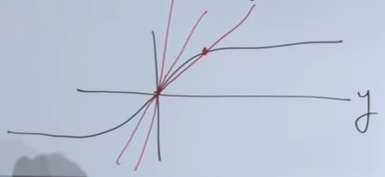
\includegraphics[width=0.8\textwidth]{tanh_mean_field}
\end{figure}

Why doesn't this work for $d=1$?

Start with T=0: everything aligned--Figure \ref{fig:T:zero:aligned}.

\begin{figure}[H]
	\centering
	\caption{Ground State, 1D}\label{fig:T:zero:aligned}
	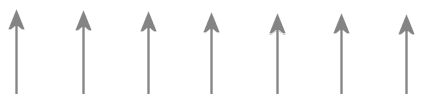
\includegraphics[width=0.7\textwidth]{T_zero_aligned}
\end{figure}

 We will compute the partition function--(\ref{eq:partition:function}). Starting from $T=0$, Figure \ref{fig:T:zero:aligned} is the dominant configuration, or in 2D, Figure \ref{fig:2d:t0}.
 
 If we flip one spin in Figure \ref{fig:2d:t0} we increase energy by 4; we can do this at any point in lattice. If we flip two spins, energy increases by 6 if the spins are adjacent--Figure \ref{fig:2d:adjacent}--or 8 if they are apart; once again, there are many ways to do this.
  
 \begin{figure}[H]
 	\caption{Two dimensional Ising Model}
 	\begin{subfigure}[b]{0.45\textwidth}
 		\centering
 		\caption{Ground State}
 		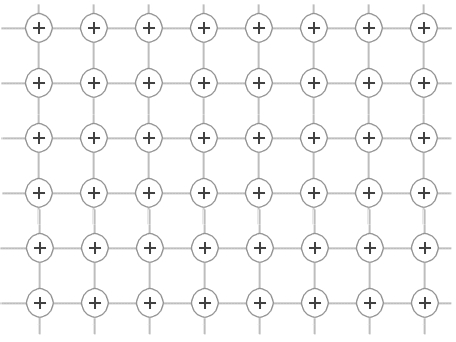
\includegraphics[width=\textwidth]{ising2D0}\label{fig:2d:t0}
 	\end{subfigure}
 	\hfill
 	\begin{subfigure}[b]{0.45\textwidth}
 		\centering
 		\caption{Flip two adjacent spins}\label{fig:2d:adjacent}
 		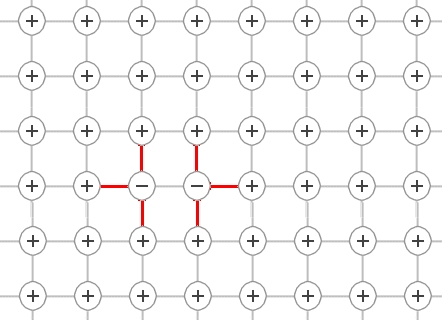
\includegraphics[width=\textwidth]{ising2D2a}
 	\end{subfigure}
 \end{figure}

Figure \ref{fig:1D:flip_adjacent} shows that we break only two bonds when any number of adjacent spins are flipped. There are therefore many states that are close to Ground State in 1d case: this is the bases of the reason why the mean field approximation doesn't work for 1D.
 
\begin{figure}[H]
	\center
	\caption{1D flip adjacent spins}\label{fig:1D:flip_adjacent}
	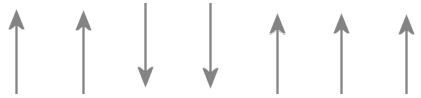
\includegraphics[width=0.7\textwidth]{T_zero_aligned_flip}
\end{figure}

Returning to 2D, lets apply a small magnetic field $B$ favouring up-spin. Then (\ref{eq:E:sigma}) becomes:
\begin{align*}
	E =& -2 d j \sigma \bar{\sigma} - B\sigma\\
	=& 	\big[-2 d j  \bar{\sigma} - B\big] \sigma \text{, and (\ref{eq:tanh_mean_field}) becomes}\\
	\frac{T y}{2 d j} =& \tanh(y +B\beta)\numberthis\label{eq:tanh_mean_field_B}
\end{align*}

Figure \ref{fig:tanh_mean_field_B} illustrates to solution to (\ref{eq:tanh_mean_field_B}). There is no longer a solution $\sigma=0$ for finite $T$.
\begin{figure}[H]
	\caption{Solving $\frac{T y}{2 d j} = \tanh(y +B\beta)$}\label{fig:tanh_mean_field_B}
	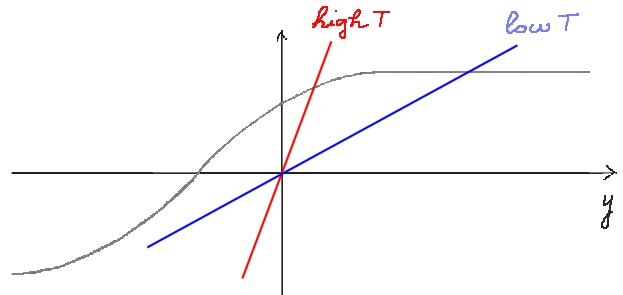
\includegraphics[width=0.9\textwidth]{tanh_mean_field_B}
\end{figure}


\section{Liquid-gas phase transition}

\subsection{Ising model continued}

We will examine the way the Ising model can be used for the liquid/gas transition. NB mean field is not accurate for 1D. 

Energy was stored in the links between sites. Unbroken bond(parallel) has low energy, broken bonds high. Every broken bond costs energy $2J$.

\begin{align*}
E =& -J \sum_{links} \sigma(i) \sigma(j) + \sum_{i}h\sigma(i)
\end{align*}

2D lattice has 2 links per site.

Ground state energy not important; it is the difference between energy levels that matters.

Our mean field equation (\ref{eq:tanh_mean_field}) becomes
\begin{align*}
\frac{ y}{2 d j \beta} =& \tanh(y - \beta h)
\end{align*}
When $h=0$, Figure \ref{fig:tanh_mean_field} shows two solution for sufficiently small T. If $h\ne0$, only one magnetization.
$T_{crit} = 2 d J$ is poor for $d=2$, good for $d=3$.

\subsection{Liquid-gas phase transition}

https://youtu.be/IWtcFAP3ju4?t=2423


\printglossaries

\end{document}
